\chapter{Engineering of Adaptive Control}\label{ch:adaptive_controller}
This chapter outlines the pertinent aspects of the \Lone adaptive control architecture used for this research.  The distinction between direct and indirect adaptive control is made in order to illustrate the importance of why the indirect architecture is critical for the \Lone algorithm.  This chapter also defines the parameter estimates provided by the \Lone algorithm with respect to the aerodynamic model simplifications outlined in Appendix~\ref{appendix:dynamics_model}.  Finally, the \Lone adaptive control filter is explained and the methods used for discretizing the algorithm for autopilot integration are discussed.  It should be noted that the versions of the \Lone adaptive controller have been patented and proper licensing should be considered if commercial use is desired.

\section{\Lone Adaptive Control}
The \Lone adaptive controller is an evolution of the concepts implemented by \ac{MRAC}.  They are similar approaches designed to control a system with unknown parameters.  The estimates of unknown parameters are adjusted to achieve the desired outcome of the error between the actual plant (system) and the referenced system model (state predictor) to asymptotically approach zero.   Adaptive control attempts to estimate the plant's unknown parameters in situ.  Parameter estimation is done using either direct or indirect architecture.  The indirect architecture attempts to estimate the system's parameters and can be compared to online system identification.  Alternately, the easier to implement direct architecture estimates the controller parameters explicitly.  These architectures can be seen in Figures~\ref{fig:direct_mrac} and \ref{fig:indirect_mrac}.

\begin{figure}[h!]
 \centering
  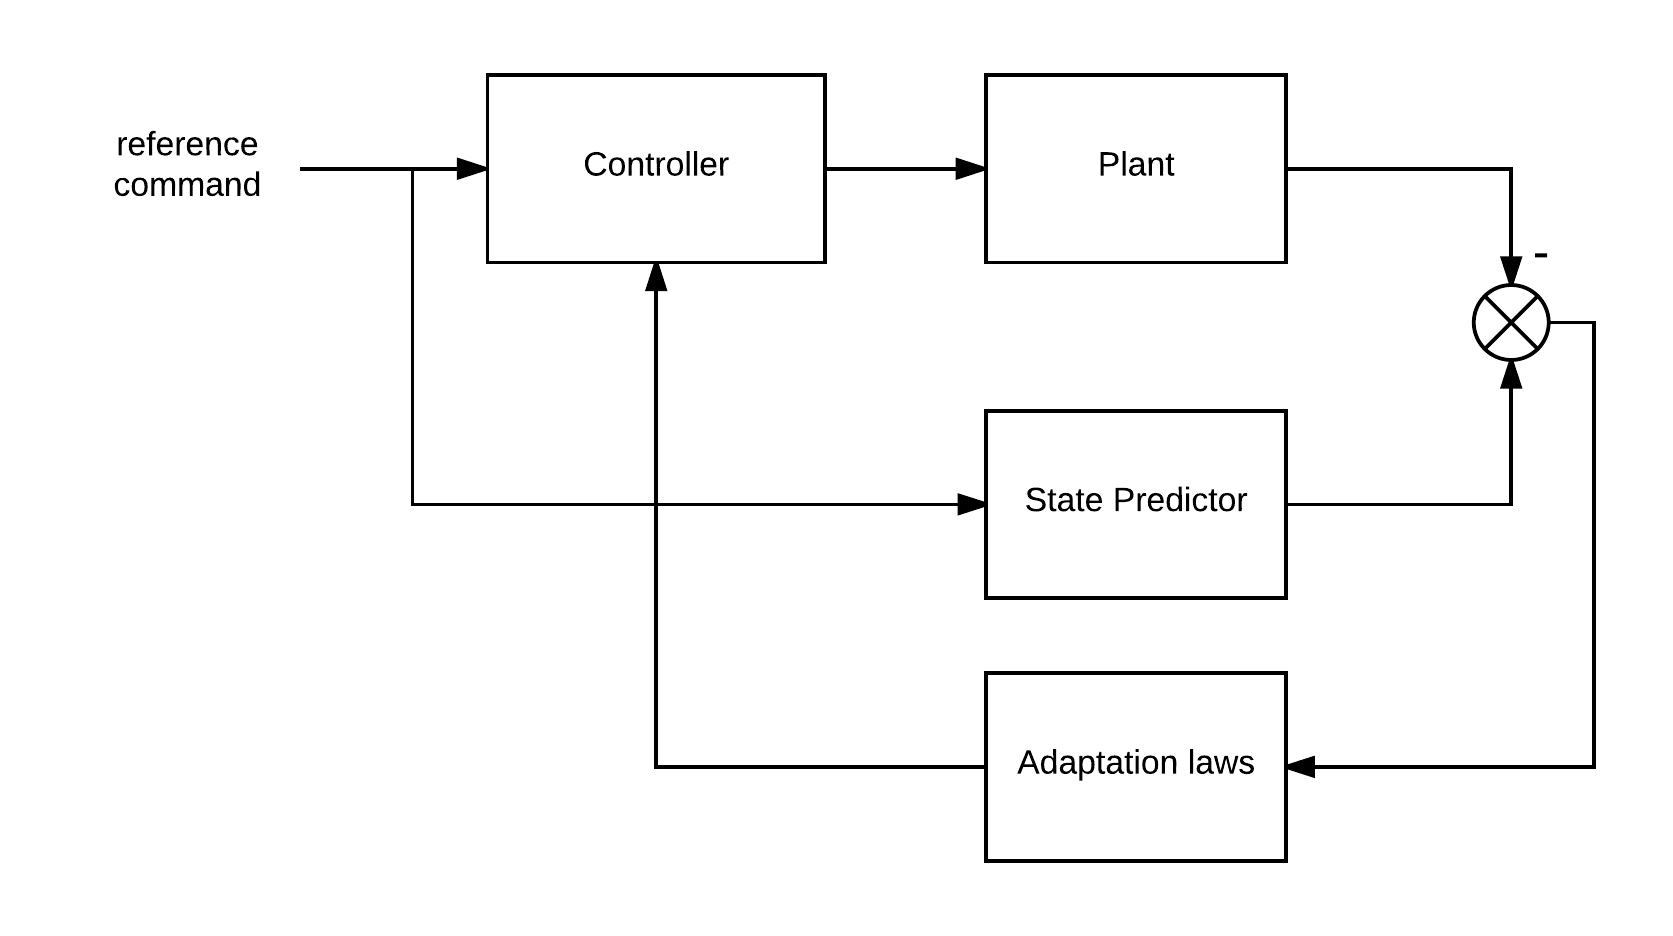
\includegraphics[width=0.75\textwidth]{Direct_MRAC.png}
  \caption{Direct \ac{MRAC} Architecture }
  \label{fig:direct_mrac}
\end{figure}

\begin{figure}[h!]
 \centering
  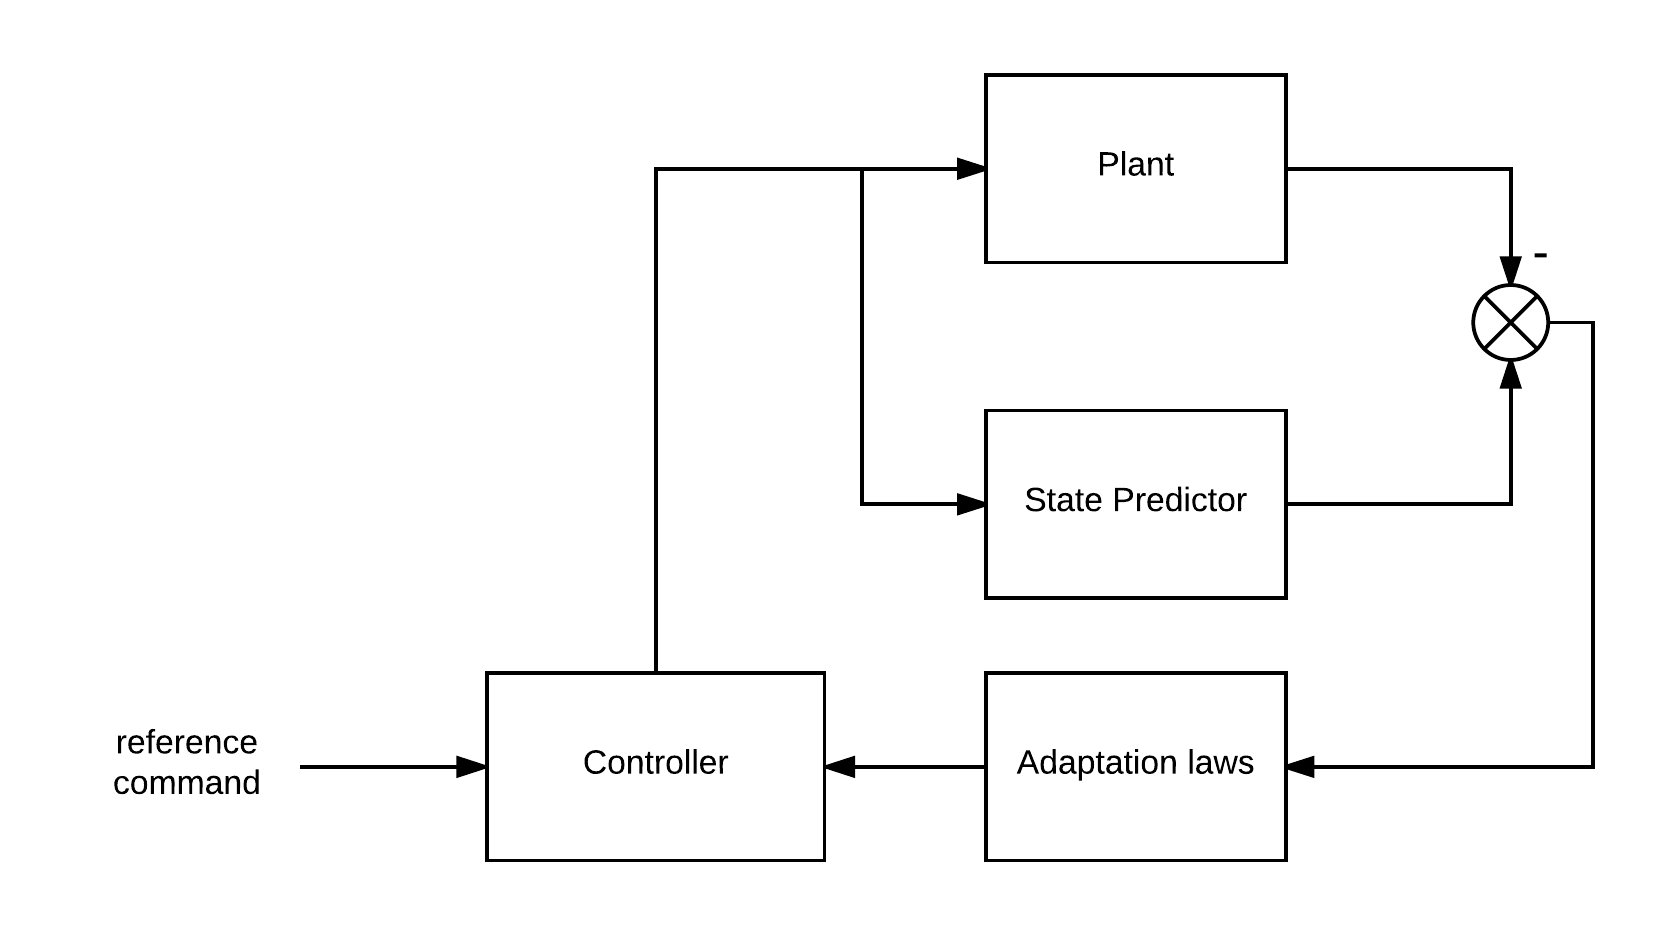
\includegraphics[width=0.75\textwidth]{Indirect_MRAC.png}
  \caption{Indirect \ac{MRAC} Architecture }
  \label{fig:indirect_mrac}
\end{figure}

\subsection{Reference Model versus Companion Model}
Traditional \ac{MRAC} controllers often refer to the system objective function as the \enquote{Reference Model.}  In this case, the engineer designs a reference model response, and it is from this model response that the error state is calculated directly.  Because the \Lone adaptive control implements the use of a filter in conjunction with a model objective function, the model is often referred to as the \enquote{Companion Model.}  This subtle distinction is necessary because the engineer must be aware that the system response will be the with respect to the filter plus the companion model in series.  In other words, the plant will not mimic the companion model; it will mimic the companion model plus the filter section.

\subsection{\Lone Architecture}
The \Lone adaptive control algorithm asserts that trying to estimate the plant uncertainties outside of the control actuators' bandwidth is overly ambitious.  The system's actuator bandwidth and the slow dynamics of the plant are most commonly the system's limiting factors, and the estimator's robustness/stability could be in question if unmodeled high-frequency content exists in the plant.  % See RHORs example here? 
The \Lone adaptive control constrains the objective function by using a low-pass filter (first or second-order) to limit the frequency response to meet robustness specifications.  This low-pass filter should be tuned to a frequency response commensurate with the actuator's frequency response.  Through inspection the low-pass filter placement in the controller topology, it becomes clear that the indirect architecture is the only candidate.  Figures~\ref{fig:direct_mrac_lowpass} and \ref{fig:indirect_mrac_lowpass} illustrate the placement of the low-pass filter and its implication on the closed loop model. 

\begin{figure}[h!]
 \centering
  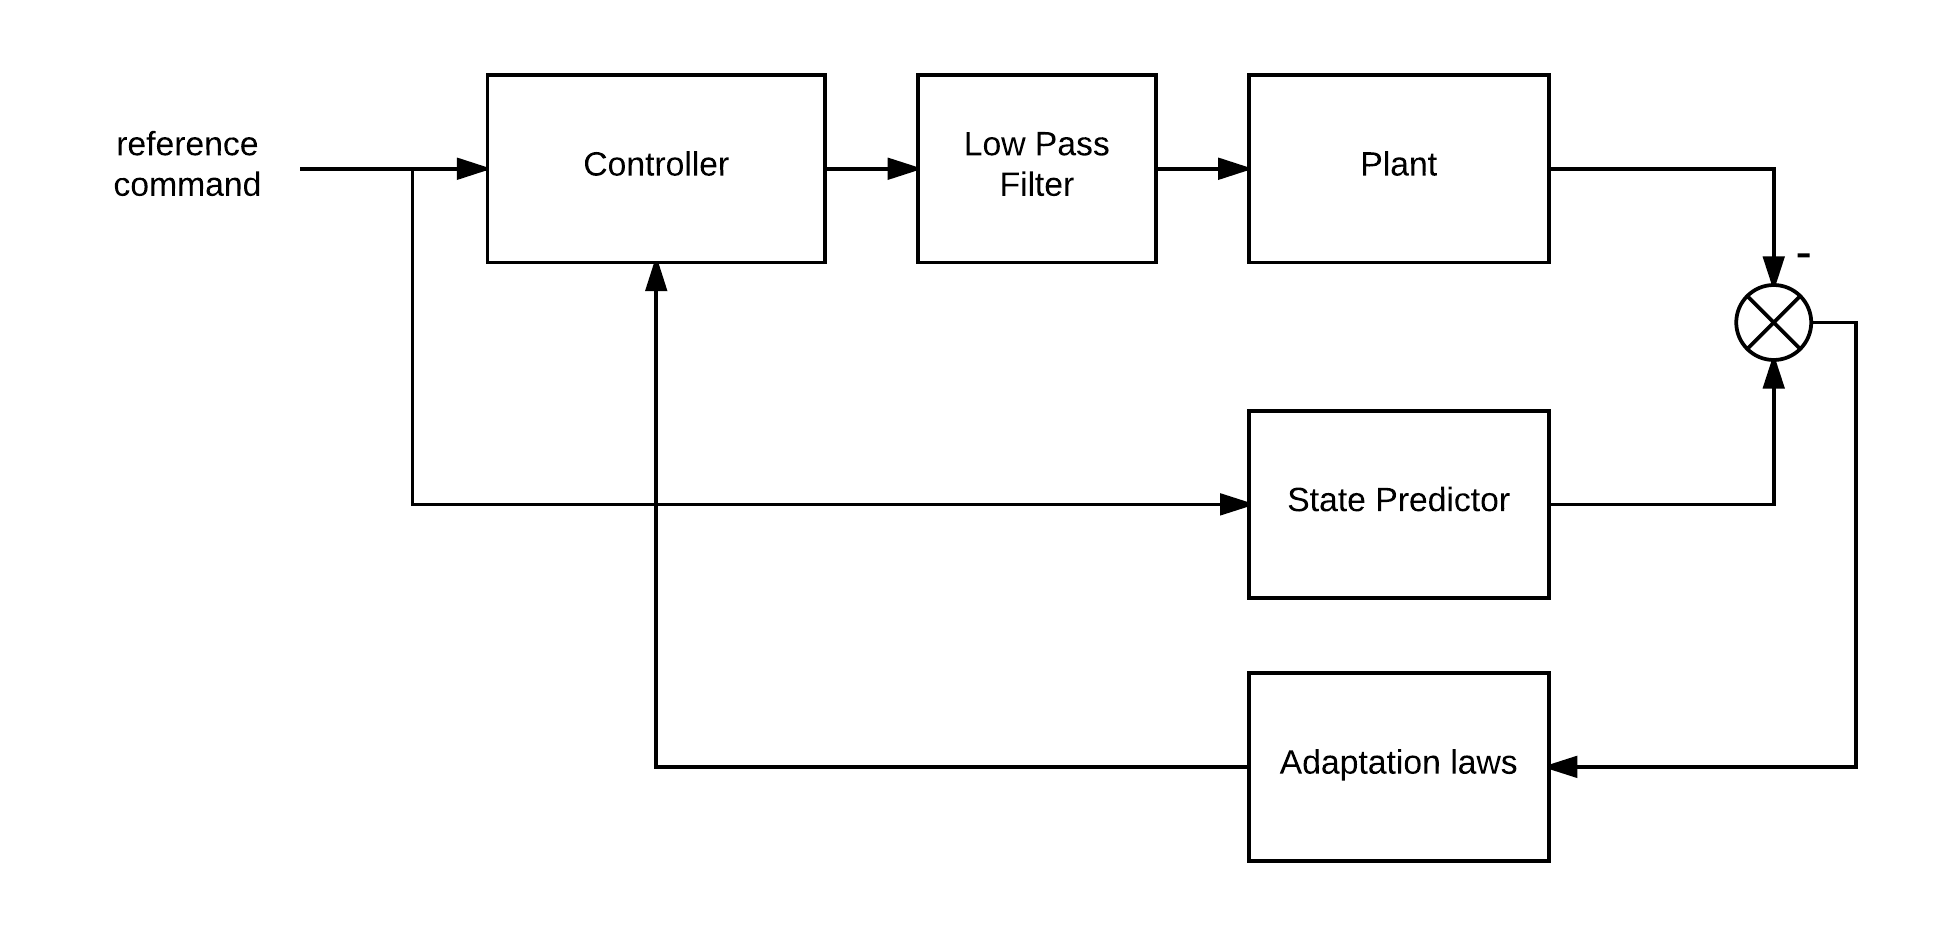
\includegraphics[width=0.75\textwidth]{Direct_MRAC_lowpass.png}
  \caption{Direct \ac{MRAC} Architecture with Low-Pass Filter }
  \label{fig:direct_mrac_lowpass}
\end{figure}
 It can be seen in Figure~\ref{fig:direct_mrac_lowpass} that the direct architecture implementation of the low-pass filter introduces difficulties.  The companion model (state predictor) is defined using aerodynamic model and the stability is verified for a Lyapunov candidate function.  However, these underpinnings designed in the companion model become nonsensical in the implementation found in Figure~\ref{fig:direct_mrac_lowpass} because of the filter is applied to the plant while is not modeled in the companion model.  This specific filter placement is non-subtractable when the error state is calculated because it is not applied in both signal paths (plant and state predictor).
\begin{figure}[h!]
 \centering
  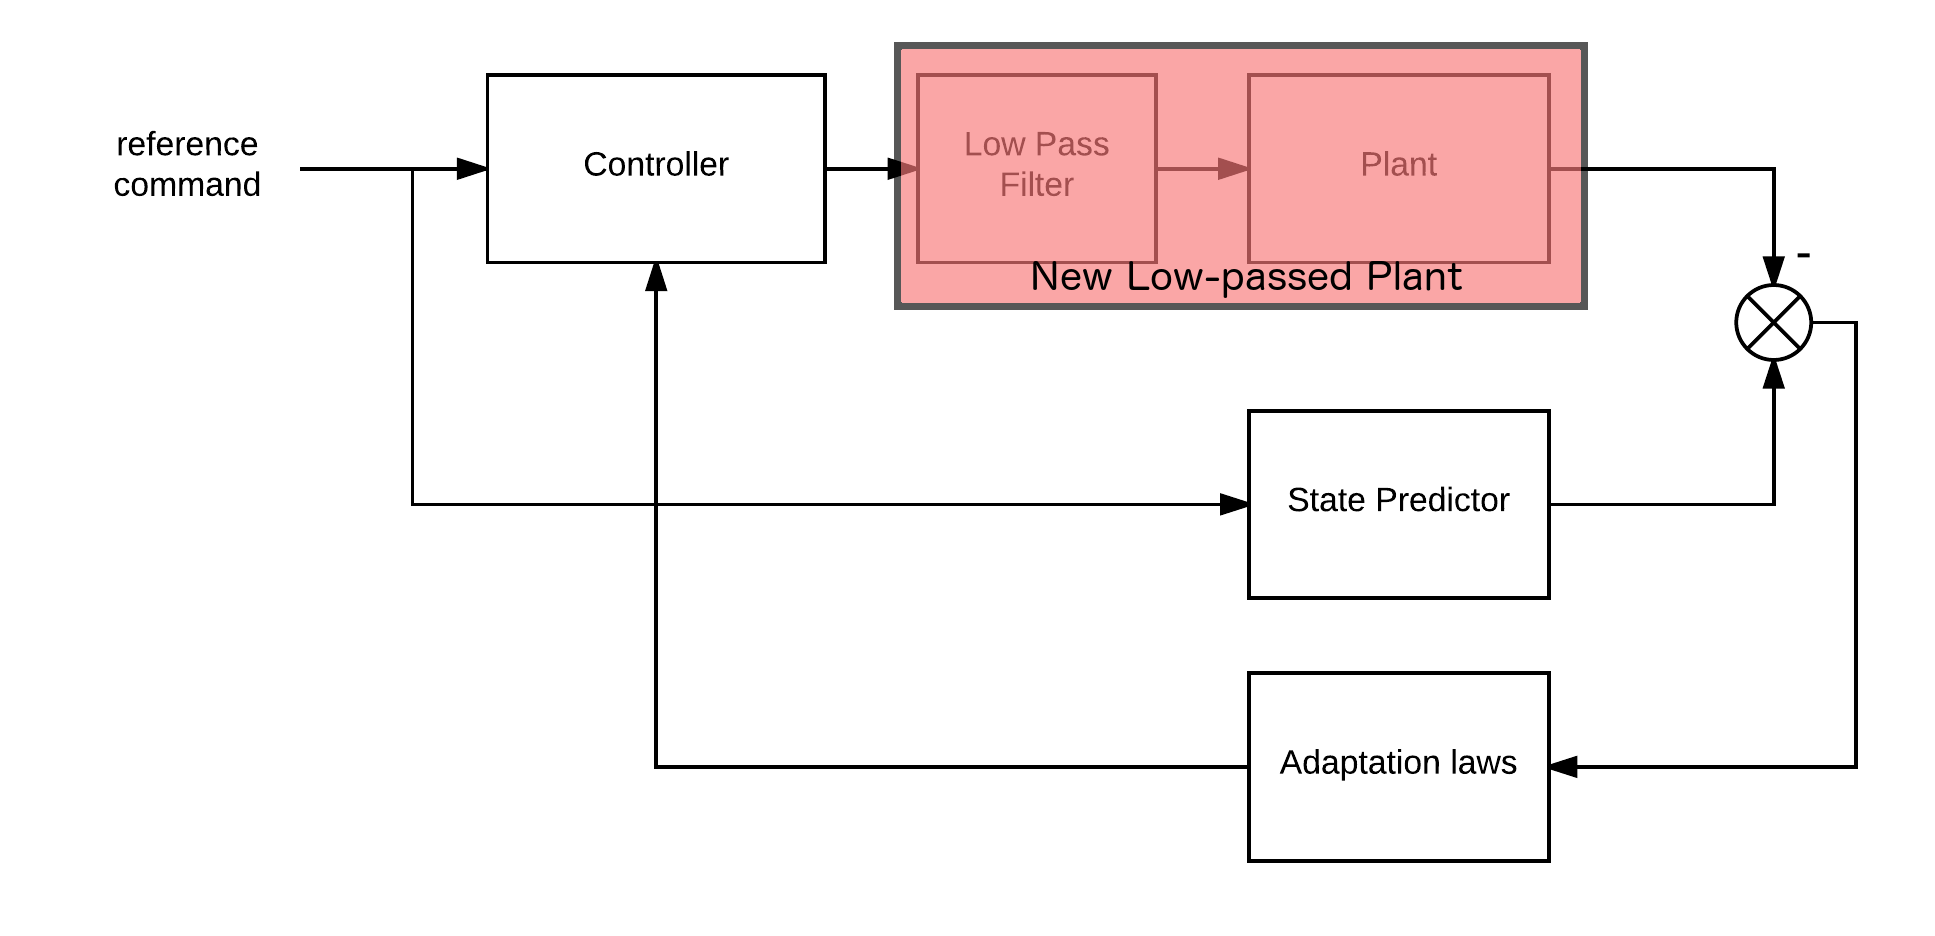
\includegraphics[width=0.75\textwidth]{Direct_MRAC_lowpass_plant.png}
  \caption{Non-Subtractable Low-Pass Implementation - Direct Architecture}
  \label{fig:direct_mrac_lowpass}
\end{figure}

Conversely, the indirect approach offers an implementation which ensures the low-pass filter is applied to both the companion model (state predictor) and the plant ensuring that the interaction of the filter is subtractable when calculating the error state.
\begin{figure}[h!]
 \centering
  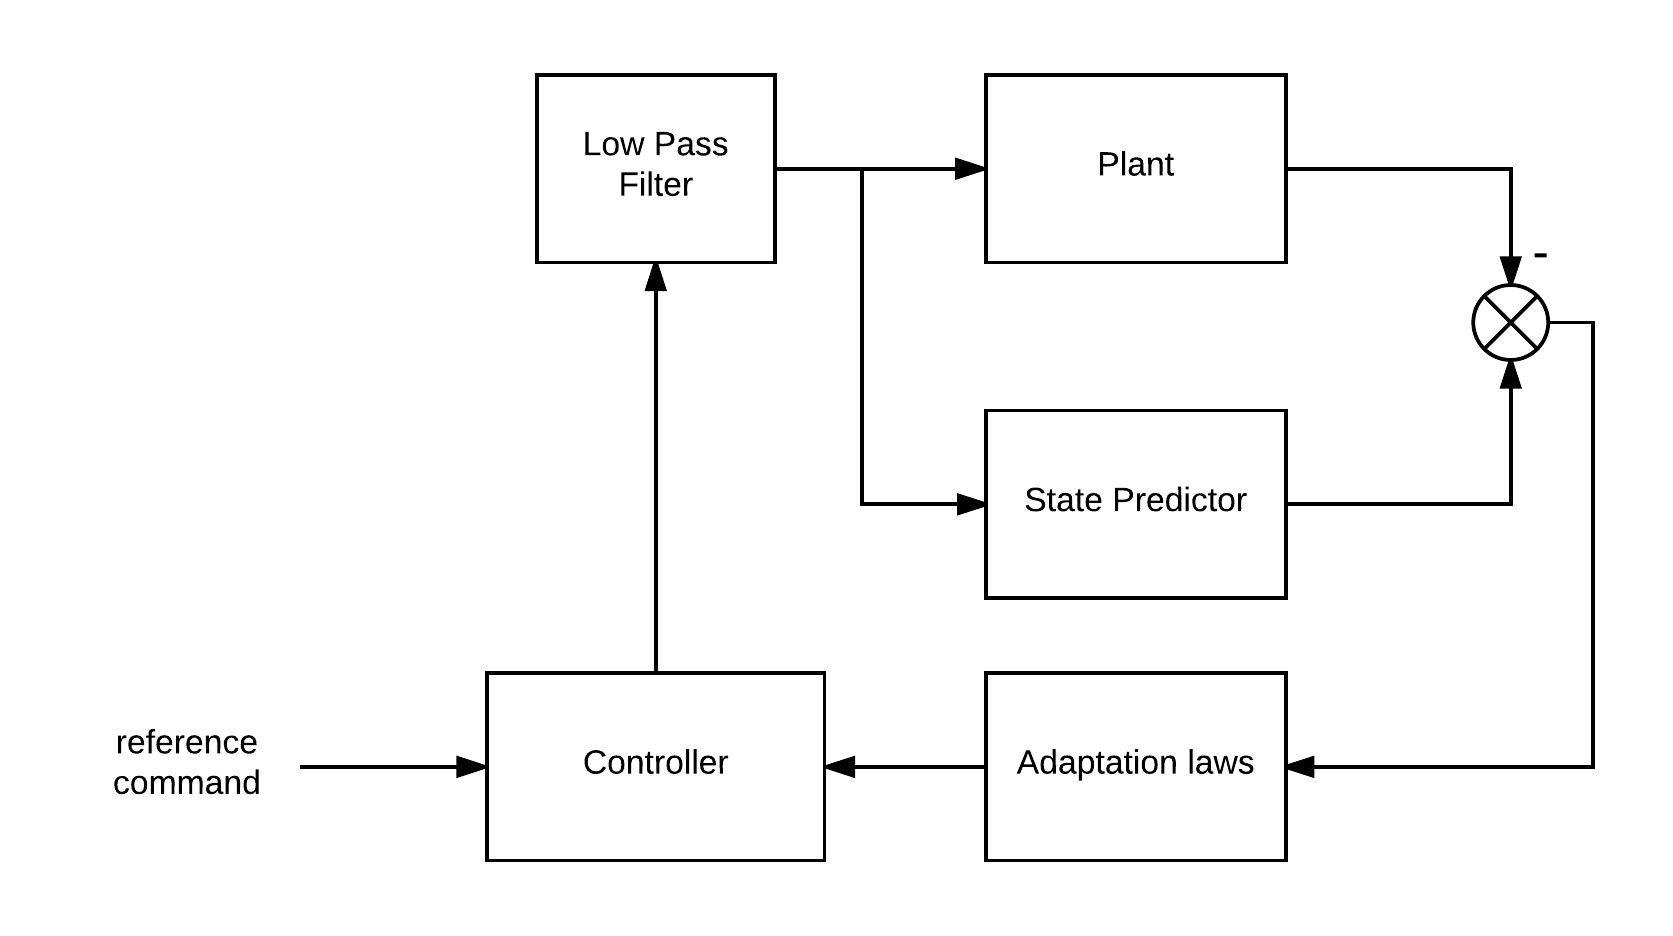
\includegraphics[width=0.75\textwidth]{Indirect_MRAC_lowpass.png}
  \caption{Indirect \ac{MRAC} Architecture with Low-Pass Filter }
  \label{fig:indirect_mrac_lowpass}
\end{figure}

It can be seen that the low-pass filter in the direct architecture inherently changes the structure of the plant with the cascading of the low-pass filter and plant block diagrams.  This change mathematically is not mirrored in the companion model (state predictor) and therefore is not subtractable.  This means that the state predictor is modeling incomplete information and therefore will incorrectly characterize the system.  However, in the indirect case, the structure of the model is kept intact, and the low-pass filter is applied to both the plant and the state predictor.  This ensures that the low-pass filter is subtractable when calculating the error state and the model's structure is kept intact.  

Many variations of the \Lone adaptive architectures have been derived for various use cases \cite{hovakimyan2010l1}.  Some of the following forms were studied for viability in the fixed wing \ac{UAS} use case with respect to state parameters $(\theta, \omega, \sigma)$ as described in Figure~\ref{fig:l1_architecture} and Section~\ref{sec:param_estimation}:
\begin{itemize}
 \item \ac{SISO} with constant but unknown state parameters
 \item \ac{SISO} with time variant and/or nonlinear unknown bounded state parameters
 \item \ac{MIMO} with constant but unknown state parameters 
 \item \ac{MIMO} with time variant and/or nonlinear unknown bounded state parameters
\end{itemize}

\ac{MIMO} control algorithms would potentially afford the controller more ability to cope with system coupling if present.  Fixed wing \ac{UAS} equations of motion, as seen in Equation~\ref{eq:aero_torques}, exhibit coupled behavior both in the aerodynamic and inertial coupling.  However, \ac{MIMO} was not chosen due to the added complexity required to architect the algorithm into source code.  Unknown state parameters that are assumed to be constant or time invariant are considered matched uncertainty.  Unknown state parameters that are non-constant (time variant) and/or exhibit non-linear behavior are considered unmatched uncertainty.  The unmatched uncertainty architecture offers a more appealing solution for fixed wing use cases (asymmetric actuator failure, aerodynamic coefficients scaled by dynamic pressure), but adds a significant amount of complexity to the architecture.  In summary, the \ac{SISO} architecture with matched uncertainty was chosen for this research.  

The \ac{SISO} controller with matched uncertainty was selected to control pitch rate $(q)$ and roll rate $(p)$ of the aircraft using two separate controllers.  The simplified equations in Equation~\ref{eq:body_rate_simplified} assume that there is no aerodynamic or inertial coupling in order to simplify the model.  This simplification was chosen to make the controller as airframe agnostic as possible while enabling very simple applications in code.  Utilizing this simplified architecture may be at the detriment of controller performance, but as seen by the flight test results in Section~\ref{sec:flight_test}, the baseline performance is adequate to achieve performance which is better than \ac{PID} in some cases.  In this implementation of the \Lone adaptive controller, the desired state $x$ to be controlled was an individual body rate (\eg $q$, $p$). 

\begin{figure}[h!]
 \centering
  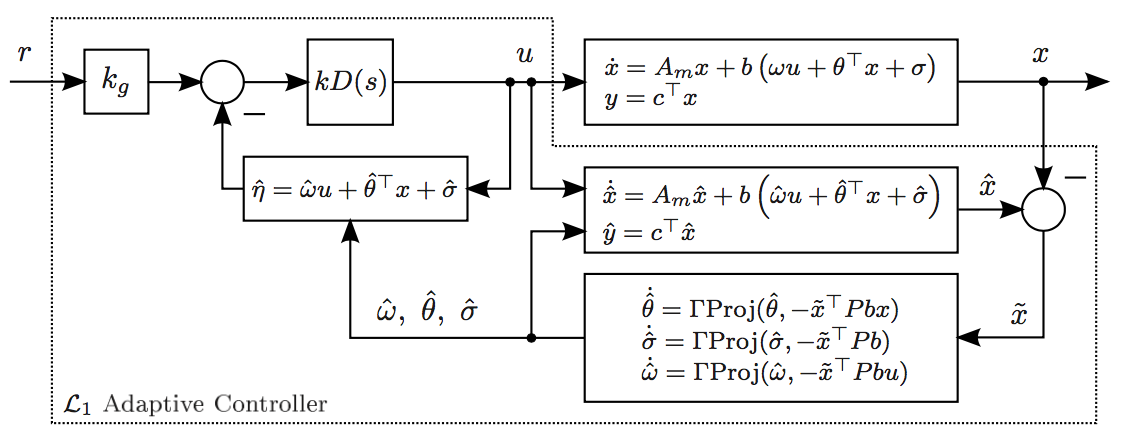
\includegraphics[width=1.0\textwidth]{L1_architecture.png}
  \caption{\Lone Architecture with Matched Uncertainty Block Diagram \cite{hovakimyan2010l1} }
  \label{fig:l1_architecture}
\end{figure}

As seen in Figure~\ref{fig:l1_architecture}, the generalized \Lone architecture in block diagram form and the following elements can be identified
\begin{itemize}
 \item[] $k_g$ - feed forward input gain
 \item[] $k$ - feedback gain
 \item[] $D(s)$ - user described filter (second-order low-pass plus integrator)
 \item[] $\hat{\eta}$ - \Lone controller state
 \item[] $\dot{x}$ - first-order differential equation of state model
 \item[] $\hat{x}$ - state estimate
 \item[] $\tilde{x}$ - state error
 \item[] $u$ - controller output
 \item[] $r$ - reference input
 \item[] $A_m$ - Hurwitz matrix
 \item[] $b$ - input matrix
 \item[] $\hat{\omega}$ - unknown input gain coefficient
 \item[] $\hat{\theta}$ - unknown constant state coefficient
 \item[] $\hat{\sigma}$ - unknown disturbance estimate
 \item[] $\Gamma$ - adaptation gain
 \item[] $Pb$ - solution to the Lyapunov stability equation 
\end{itemize}

It should also be noted that the architecture presented in Figure~\ref{fig:l1_architecture} includes the use of a projection operator.  The estimation dynamics of $\dot{\hat{\omega}}$, $\dot{\hat{\theta}}$, and $\dot{\hat{\sigma}}$ are projection based adaptation laws.  This ensures that the adaptation stays bounded around the feasible region of parameter space.  The Lyapunov stability proofs for this architecture rely on this method to guarantee stability\cite{hovakimyan2010l1}.  More discussion on the specific implementation of this operator can be found in Appendix~\ref{appendix:projection_derivation}.

One of the main benefits of using the \ac{SISO} architecture is in its simplicity so that the solution to the Lyapunov stability equation ($Pb$) utilized in the projection based adaptation laws is greatly simplified.  

In this case, $Pb$ reduces to:
\begin{equation}
Pb = \frac{1}{2\omega_n}
\end{equation}

where $\omega_n$ is the natural frequency in rad/s for the first-order companion model in discrete recursive form assuming DC gain of 1.  The proof for this can be found in Appendix~\ref{sec:projection_proof}.

%---------------------------------------------------
\section{\Lone Parameter Estimation}\label{sec:param_estimation}
Three model parameters were evaluated in this research.   The first model parameter $\theta$ establishes the baseline architecture and Lyapunov stability proof.  Each additional  model parameter added to the architecture adds complexity to the architecture and its required stability proofs.  The general progressive build up of the three parameter architecture is outlined in the nomenclature for the estimation of a system with unknown constant parameters, input/output disturbances, and an unknown system input gain.

The \Lone adaptive control algorithm is primarily used to estimate unknown constant system parameters.  These system parameters are defined as $\theta$ as seen in the following model:
\begin{equation}
\dot{x}(t)=Ax(t)+b(u(t)+\theta^{\top}(t)x(t))
\end{equation}

The second adaptive element is the estimation of the input/output disturbances $(\sigma)$.  This additional parameter is implemented in this research as any unmodeled transient dynamics such as aerodynamic/inertial coupling.  This model takes the form
\begin{equation}
\dot{x}(t)=Ax(t)+b(u(t)+\theta^{\top}(t)x(t)+\sigma(t))
\end{equation}

The last adaptive element used for this research was the estimation of unknown system input gain $(\omega)$.  Estimating the unknown system input gain offers the controller the ability to estimate the actuator effectiveness for changes in dynamic pressure or failed control surfaces.  This model takes the form
\begin{equation}\label{eq:l_one_model}
\dot{x}(t)=Ax(t)+b(\omega(t)u(t)+\theta^{\top}(t)x(t)+\sigma(t))
\end{equation}  

The model in Equation~\ref{eq:l_one_model} can be paralleled to the aircraft model derived in Equation~\ref{eq:simplified_ac_model}.  As a result, the roll rate model takes the similar form

\begin{equation}
 \hat{\dot{p}}=A_p\hat{p}+b_p\left(\hat{\omega}_p\delta_a+\hat{\theta}_pp+\hat{\sigma}_p\right)
\end{equation}

This final model, with the inclusion of all three estimated parameters $(\hat{\omega}, \hat{\theta}, \hat{\sigma})$, established the architecture tested in this research.  The fundamental assumption that the aerodynamic and inertial coupling was negligible and set to zero as outlined in Equation~\ref{eq:body_rate_simplified} is agreeably a gross assumption which may prove to be inadequate for stable flight.  These assumptions presume that the estimated input/output disturbance $(\hat{\sigma})$ would be adequate to compensate for these unmodeled dynamics and were validated by successful flight test in Section~\ref{sec:flight_test}.  

These derivations of the \Lone algorithm guarantees that the error between the model and plant asymptotically approaches zero, but this does not imply the constraint that the estimated parameters are in fact converging to their real values.  The algorithm only guarantees that the parameters are bounded and therefore it is common to observe the parameters never reaching steady-state.  The engineer must ensure that the bounds set on the parameters are sufficient for the controlled system to not become unstable.  In the discrete form, the algorithm can have numerical floating point instability if these projection operator bounds are too high and not thoroughly tested in simulation.

%---------------------------------------------------
\section{\Lone Filter - $C(s)$}\label{sec:l1_filter}
One of the key features of the \Lone adaptive controller is that the robustness of the controller is decoupled from the adaptation rate.  This is handled in the filter section of the \Lone architecture which is annotated as $C(s)$.  To ensure guaranteed stability of the \Lone algorithm, $C(s)$ must be verified as strictly-proper stable.  With the architecture that includes the system input gain $(\omega)$, one cannot simply apply a stand alone filter.  The inclusion of $\omega$ in the architecture block diagram in Figure~\ref{fig:l1_architecture} slightly modifies the signal output and takes the following form
\begin{equation}
u(s)=-kD(s)(\hat{\eta}(s)-k_gr(s))
\end{equation}
where $D(s)$ is the new user defined filter and $C(s)$ now takes the form
\begin{equation}
\begin{split}
\omega \in \Omega_0 \triangleq [\omega_{l_0},\omega_{u_0}]\\
C(s)=\frac{\omega kD(s)}{1+\omega kD(s)}
\end{split}
\end{equation}

In the case which the user defined function $D(s)$ is a simple integrator, $C(s)$ takes the form
\begin{equation}\label{eq:l1_filter}
\begin{split}
D(s)&=\frac{1}{s}\\
C(s)&=\frac{\omega k}{s+\omega k}
\end{split}
\end{equation}

The feedback gain $k$ should not be assumed to be 1 in this case.  As seen in Equation~\ref{eq:l1_filter}, the $C(s)$ transfer function is a function of $k$ that can have significant influence on the controller output.  In actual implementation, $k$ was found to be one of the most influential gains in the architecture and extremely critical in specifying the transition between robustness and performance.


%---------------------------------------------------
\section{\Lone Discrete Time Implementation}\label{sec:discrete_time_implementation}
Implementing any algorithm on actual autopilot hardware will inevitably force some if not all parts of the algorithm to be discretized.  Autopilots like the Pixhawk operate at some scheduled loop rate for executing the litany of subprograms that measure sensors, calculate navigation commands, and much more.  In the case of the Pixhawk autopilot, the main loop can run up to 400 Hz.  At a 400 Hz sampling rate, there is a significant insurance that the vehicle's dynamics bandwidth will be completely defined.  However, the \ac{APM} flight stack records all logged parameters also at this loop rate and can create log files larger than are reasonably desired.  There are a myriad of other reasons why the engineer would not want to run at high loop rates, but successful flight at the lowest (default of 50 Hz) is desired if adequate performance of the adaptive control can be achieved.  Failures in early adaptive control were largely in part due to a very naive understanding of robustness.  Brian Anderson concludes that \enquote{it is clear that the identification time scale needs to be faster than the plant variation time scale, else identification cannot keep up} \cite{anderson2005failures}.  

The \Lone architecture does not require the algorithm to run in sync with the sensor measurements.  Ideally, the autopilot main loop rate would remain at its default value (50 Hz), and the adaptation section of the \Lone controller would run as fast as the CPU would allow.  However, the \ac{APM} architecture does not lend itself well to this scheme in its current configuration without significant modification to the code base.  Therefore, the initial tests presumed that the \Lone algorithm is running at the same frequency as the main loop of the autopilot.  The fundamental derivation of the \Lone algorithm proves that performance and adaptation gain are maximized as the loop time $(dt)$ approaches zero.  Increased performance would come from higher adaptation loop rates, but the primary focus was to implement the \Lone algorithm with minimal or no detrimental effects to the current \ac{APM} codebase.

\subsection{Digital Bi-Quad Filter}

The \Lone adaptive control algorithm utilizes two specific elements that will require careful discretization; the companion model and the low-pass filter.  The digital bi-quad filter offers a very versatile and straightforward method for accurately implementing the companion model and the low-pass filter discretely using its recursive nature.  It is a second-order filter which uses a \ac{FIR} front end and an \ac{IIR} back end requiring four total memory blocks.  This topology allows the designer to create numerous types of filters (low-pass, high-pass, band-pass) simply by choosing appropriate coefficients.  If a first-order filter is needed, then the higher order FIR/IIR terms can be set to zero.  Figure~\ref{fig:bi-quad} illustrates this filter's topology where the \ac{FIR} structure is the left two memory blocks and the \ac{IIR} structure is the right two memory blocks.

\begin{figure}[h!]
 \centering
  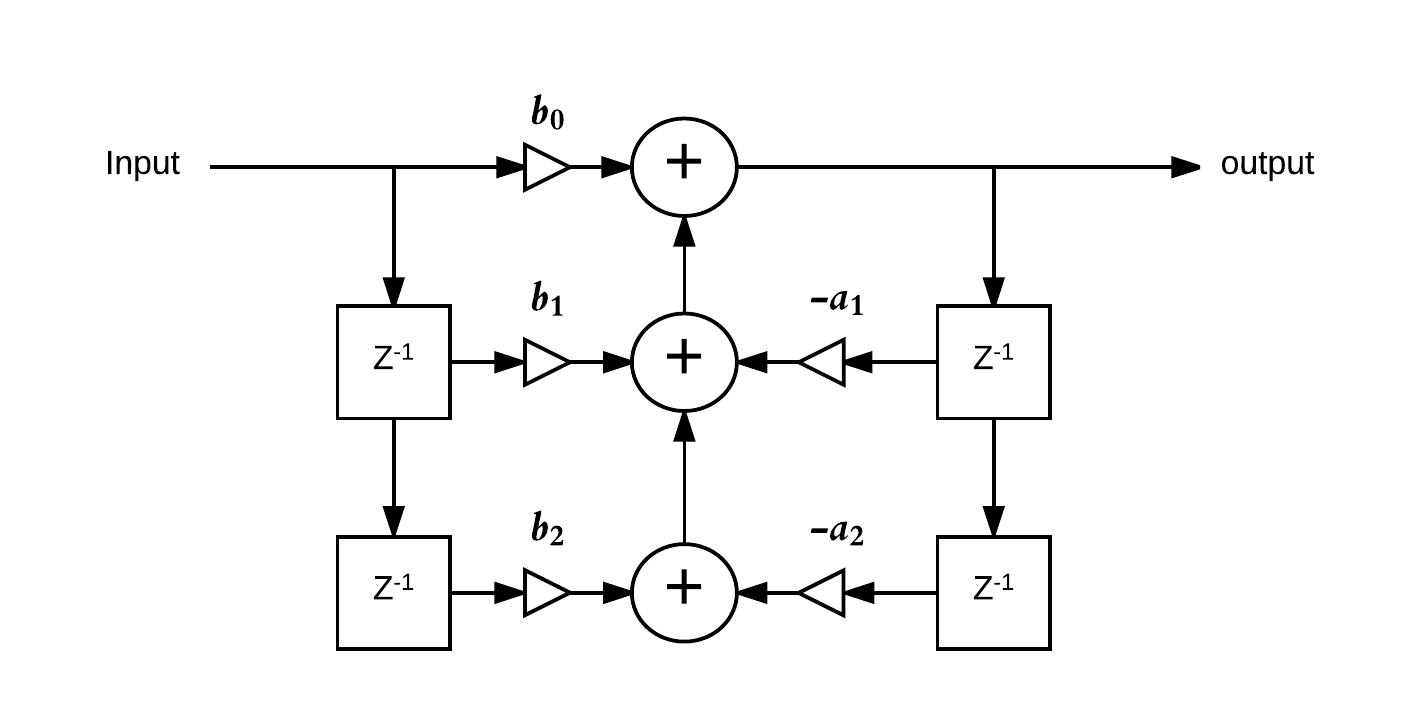
\includegraphics[width=1.0\textwidth]{bi-quad_filter.png}
  \caption{Digital Bi-quad Filter Architecture }
  \label{fig:bi-quad}
\end{figure}

A bilinear Z transform is used to convert the desired S-domain (continuous time domain) filter/model into the Z-domain (discrete time domain) to determine the structure of the coefficients.

\begin{figure}[h!]
 \centering
  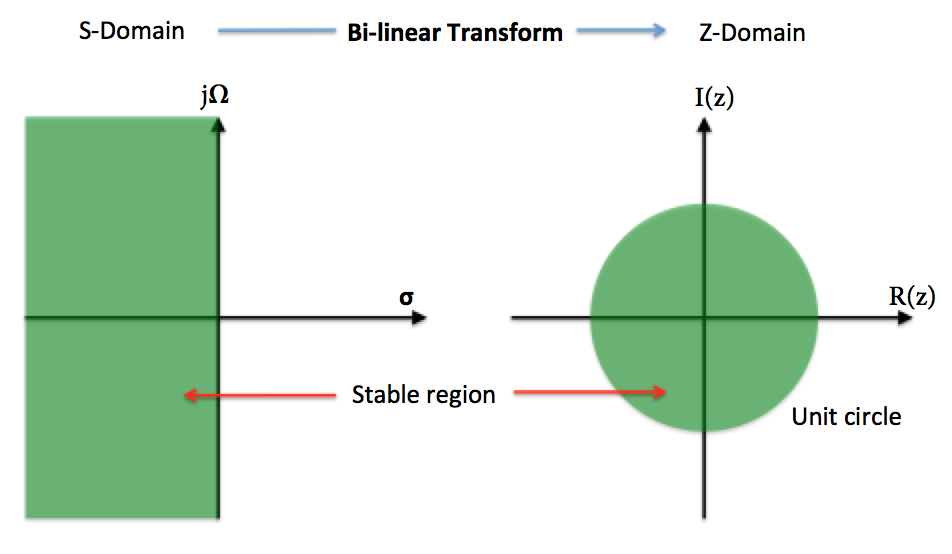
\includegraphics[width=1.0\textwidth]{bi-linear_transform.png}
  \caption{Bi-linear Transform}
  \label{fig:bi-linear_transform}
\end{figure}

This derivation for the second-order low-pass model is

\begin{equation}
 H(s) = \frac{1}{s^2+\frac{s}{Q}+1}
\end{equation}

where the bi-linear transform converts s to z via

\begin{equation}
 s = \left(\frac{1}{K}\right)\left(\frac{z-1}{z+1}\right)
\end{equation}

$K$ is the \enquote{pre-warping} factor which accounts for the transition of the vertical s-plane into the circular z-plane as seen in Figure~\ref{fig:bi-linear_transform}.

where $\omega T$ is

\begin{equation}
 \omega T = 2\pi\left(\frac{F_c}{F_s}\right)
\end{equation}

\begin{equation}
\begin{split}
 K &= tan\left(\frac{\omega T}{2}\right) \\
 &= tan\left(\pi\frac{F_c}{F_s}\right)
\end{split}
\end{equation}



$F_c$ is the desired corner frequency of the filter and $F_s$ is the sampling rate (or loop rate of the autopilot).
This \enquote{pre-warping} is critical to ensure that the continuous time cutoff frequency desired is correctly established in the discrete implementation.  It is the engineer's discretion if pre-warping is required for the appropriate application, but the general guidance is to pre-warp the Z-domain coefficients if the desired cut-off frequency is close to Nyquist–Shannon sampling theorem frequency $(\frac{F_s}{2})$.  It was chosen for this application to always pre-warp the coefficients even though the error is small for corner frequencies which are fairly distant from Nyquist–Shannon sampling theorem frequency.  Continuous calculation of the pre-warp coefficient was chosen because calculating the $tan()$ function real time on the CPU adds negligible computational strain but offers ease of tuning for the engineer.

Applying the bi-linear transform to the continuous time second-order low-pass filter results in

\begin{equation}\label{eq:bi-linear}
 H(z) = \frac{1}{ \left[\left(\frac{1}{K}\right)\left(\frac{z-1}{z+1}\right)\right]^2+\frac{ \left(\frac{1}{K}\right)\left(\frac{z-1}{z+1}\right)}{Q}+1}
\end{equation}

The desired form is

\begin{equation}\label{eq:bi-quad}
 H(z) = \frac{b_0 + b_1 z^{-1} + b_2 z^{-2}}{a_0 + a_1 z^{-1} + a_2 z^{-2}}
\end{equation}

Reducing Equation~\ref{eq:bi-linear} to match the form in Equation~\ref{eq:bi-quad} results in the following coefficients

\begin{equation}
\begin{split}
 a_0 &= 1 \\
 a_1 &= \frac{2(K^2-1)}{K^2+\frac{K}{Q}+1} \\
 a_2 &= \frac{K^2-\frac{K}{Q}+1}{K^2+\frac{K}{Q}+1} \\
 b_0 &= \frac{K^2}{K^2+\frac{K}{Q}+1} \\
 b_1 &= 2b_0 \\
 b_2 &= b_0  
\end{split}
\end{equation}

The bandwidth of the filter $Q$ can be set by the engineer.  For example, if the pass-band of the filter is desired to be flat (Butterworth) then $Q$ can be set equal to $\frac{1}{\sqrt{2}}$.  For this research, the following C++ code segments were used to explicitly calculate the bi-quad low-pass filter implementation \cite{apm_source_code}: \newline

\begin{lstlisting}[language=c++]
void DigitalBiquadFilter<T>::compute_params(float sample_freq, 
float cutoff_freq, biquad_params &ret) {
    ret.cutoff_freq = cutoff_freq;
    ret.sample_freq = sample_freq;

    float fr = sample_freq/cutoff_freq;
    float K = tanf(M_PI/fr);  //Pre-Warp calculation
    float c = 1.0f+2.0f*cosf(M_PI/4.0f)*K + K*K;

    ret.b0 = K*K/c;
    ret.b1 = 2.0f*ret.b0;
    ret.b2 = ret.b0;
    ret.a1 = 2.0f*(K*K-1.0f)/c;
    ret.a2 = (1.0f-2.0f*cosf(M_PI/4.0f)*K+K*K)/c;
}
\end{lstlisting}

\begin{lstlisting}[language=c++]
T DigitalBiquadFilter<T>::apply(const T &sample, 
const struct biquad_params &params) {
    
    T delay_element_0 = sample - _delay_element_1 * params.a1 
     - _delay_element_2 * params.a2;
    
    T output = delay_element_0 * params.b0 
     + _delay_element_1 * params.b1 
     + _delay_element_2 * params.b2;

    _delay_element_2 = _delay_element_1;
    _delay_element_1 = delay_element_0;

    return output;
}

\end{lstlisting}

This implementation can be employed as the \Lone low-pass filter and as the companion model.  It can be seen in the code segment that $K$, the pre-warp factor, is explicitly calculated every iteration.

\subsection{Simplified Bi-quad First-order Model}

In the case of the companion model, a first-order response may be desired.  As described in equations~\ref{eq:first_order_model} and \ref{eq:state_space_model}, the discrete first-order model can be derived from a simplified Bi-quad as seen in Figure~\ref{fig:bi-quad_first_order}.  It can be seen that the first coefficient of the \ac{IIR} filter is kept from this topology.
\begin{figure}[h!]
 \centering
  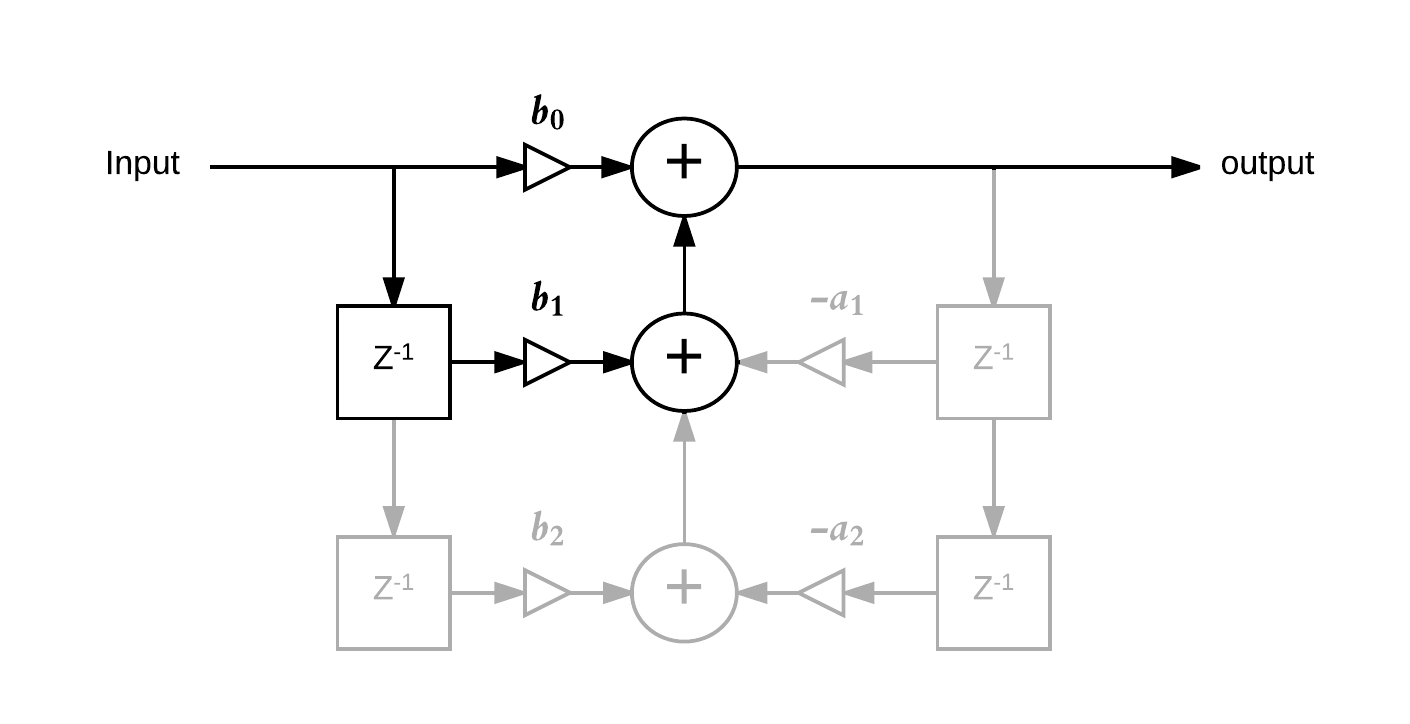
\includegraphics[width=1.0\textwidth]{bi-quad_first_order.png}
  \caption{Digital Bi-quad Simplified First-Order Low-Pass Filter }
  \label{fig:bi-quad_first_order}
\end{figure}

The first-order model can be specified by either its time constant (time in seconds to reach 63\% of steady-state) or its -3dB corner frequency.  The system takes the form as seen in Equation~\ref{eq:first_order_corner_model} when defined by its corner frequency

\begin{equation}\label{eq:first_order_corner_model}
H(s)=\frac{\omega_n}{s+\omega_n}
\end{equation}

Therefore, the explicit calculation of the Bi-quad coefficients in this case becomes

\begin{equation}\label{eq:first_order_coeffieicnts}
\begin{split}
 a_1&=e^{\left(\frac{-\omega_n}{F_s}\right)}  \\
 b_0&=1-a_1
\end{split}
\end{equation}

where $\omega_n$ is the -3dB corner frequency in radians per second and $F_s$ is the sampling frequency measured in Hertz.

Therefore, the discrete recursive form of the first-order model becomes

\begin{equation}
y_{i+1}=a_1y_{i-1}+b_0y_i
\end{equation}

Another form designed to optimize for speed that is commonly seen in software is

\begin{lstlisting}
float b_0=exp(-f_c/f_s);
float out+=(in-out)*b_0;
\end{lstlisting}

\subsection{Euler vs. Trapezoid Rule}

The model estimate, as well as the parameter estimates for the \Lone algorithm, are both numerically estimated using discrete integration.  The Euler method is a numerical procedure for solving ordinary differential equations. The Euler method as applied to discrete integration is the fundamental method for recursively integrating a digital signal.  The algorithm takes the form: \newline
where $h$ is the uniform step size,
\begin{equation}
y_{i+1}=y_i+hf(t_i,y_i)
\end{equation}

The recursive trapezoidal method takes the form
\begin{equation}\label{eq:trapezoidal_integration}
\begin{split}
\tilde{y}_{i+1}&=y_i+hf(t_i,y_i) \\
y_{i+1}&=y_i+\frac{h}{2}[f(t_i,y_i)+f(t_{i+1},\tilde{y}_{i+1})]
\end{split}
\end{equation}

Comparing the accuracy of the two numerical methods for discretely calculating the integral of $y=e^t$ can be seen in Figure~\ref{fig:trapezoidal_integration}

\begin{figure}[h!]
 \centering
  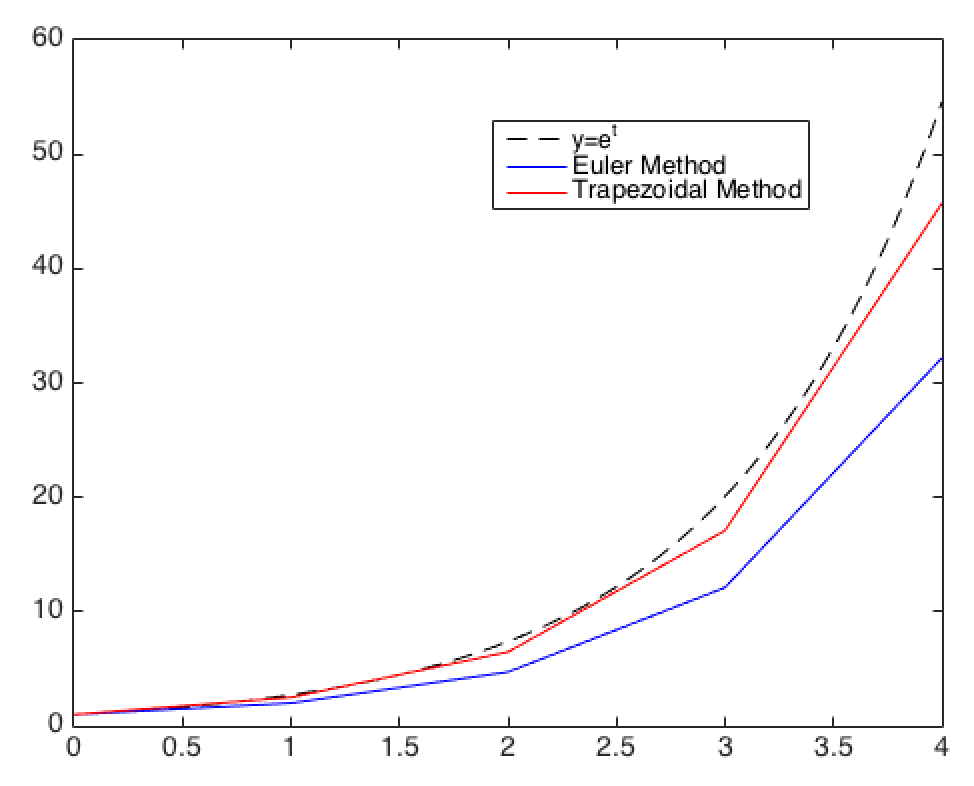
\includegraphics[width=0.75\textwidth]{trapezoidal_integration.png}
  \caption{Euler vs Trapezoidal Integration Error}
  \label{fig:trapezoidal_integration}
\end{figure}

As seen in Equation~\ref{eq:trapezoidal_integration}, the recursive trapezoidal integration method only adds one more line of complexity to the algorithm for a significant gain in accuracy and therefore will be the chosen method applied for all discrete numerical integration in this research and takes the form \newline

\begin{lstlisting}
float trap_integration(float y0, float y1_dot, float dt, float &y0_dot)
{
    float y1 = y0 + (dt/2)*(y0_dot+y1_dot);
    y0_dot = y1_dot;

    return y1;
}
\end{lstlisting}

With the \Lone adaptive control algorithm defined in discrete form utilizing the architecture in Figure~\ref{fig:l1_architecture} and the discretization methods outlined in Section~\ref{sec:discrete_time_implementation} enabled the simulation testing found in Chapter~\ref{ch:performance}.  Flight testing was also desired and therefore multiple test aircraft were designed and built as seen in Chapter~\ref{ch:platform} with integrated \ac{COTS} autopilots.











